%%================================================
%% Filename: chap05.tex
%% Encoding: UTF-8
%% Author: 苏峻锋
%%================================================
\chapter{预测模型与传统负载均衡的结合}
回顾第二章的讨论,我们已经详细分析了传统负载均衡策略的工作原理,虽然这些传统策略在多种场景下都能提供稳定的性能,但在面对动态变化和未预见负载的情况时,仍然显得力不从心。本章旨在探讨一种新的解决方案,即预测模型与传统负载均衡的结合,以期望克服现有方法的不足。我们将首先介绍结合方案的设计理念与实施策略,随后通过实验验证其有效性,并对模型的表现进行深入分析。

\section{传统负载均衡算法的选取}
在第二章的讨论中,发现了加权轮询算法原理简单,而且配置比较简便,权重可以很好的反映出集群内服务器节点的性能和负载情况,是一种非常经典的负载均衡算法。本文选择以加权轮询算法为基础,分析其原理并进行改进,实现一种检测服务器节点负载状况,并以此为根据动态地调整各个节点权重以合理分配请求任务目的的算法。

相比于默认的轮询算法,加权轮询算法则考虑了不同性能特点的服务器节点,性能好的服务器则设置较大的权值,
性能不好的服务器则设置较小的权值。
当任务入队列时负载均衡器则可以按照设置好的权值比例合理的悬着服务器执行任务请求。

在阅读 Nginx 源代码期间,发现在 ngx\_http\_upstream\_round\_robin.c 文件中的 ngx\_http\_upstream\_get\_round\_robin\_peer 函数负责实现加权轮询算法。
该算法在分配任务时使用了四个关键变量来记录上游集群服务器节点的权重状态,这些变量分别是:weight、effective\_weight、total 和 current\_weight。

\noindent\begin{longtblr}
	[caption = {加权轮询算法变量及描述}]
	{hlines, colspec = {|X[1, c]|X[2, c]|}}
	变量                & 描述        \\
	weight            & 初始权值,固定不变 \\
	effective\_weight & 发生错误,权值减小 \\
	total             & 集群服务器权值总和 \\
	current\_weight   & 实时权值,初始为零 \\
\end{longtblr}

在一个请求的处理周期中,负载均衡器会尝试将每个上游服务器节点的 current\_weight 增加其对应的 effective\_weight,
接着选择 current\_weight 最高的服务器节点作为当前任务的最合适候选。
当一个服务器节点被选中并正在处理任务时,其 current\_weight 将会相应减少。
Nginx 使用两种状态标志以表示过程的结果——NGX\_OK 表示已成功选出最适服务器,而 NGX\_BUSY 表示服务器的选取失败或发生了通信错误。
加权轮询算法详细流程如下图\ref{weight_round}所示。

\begin{figure}[htb]
	\centering
	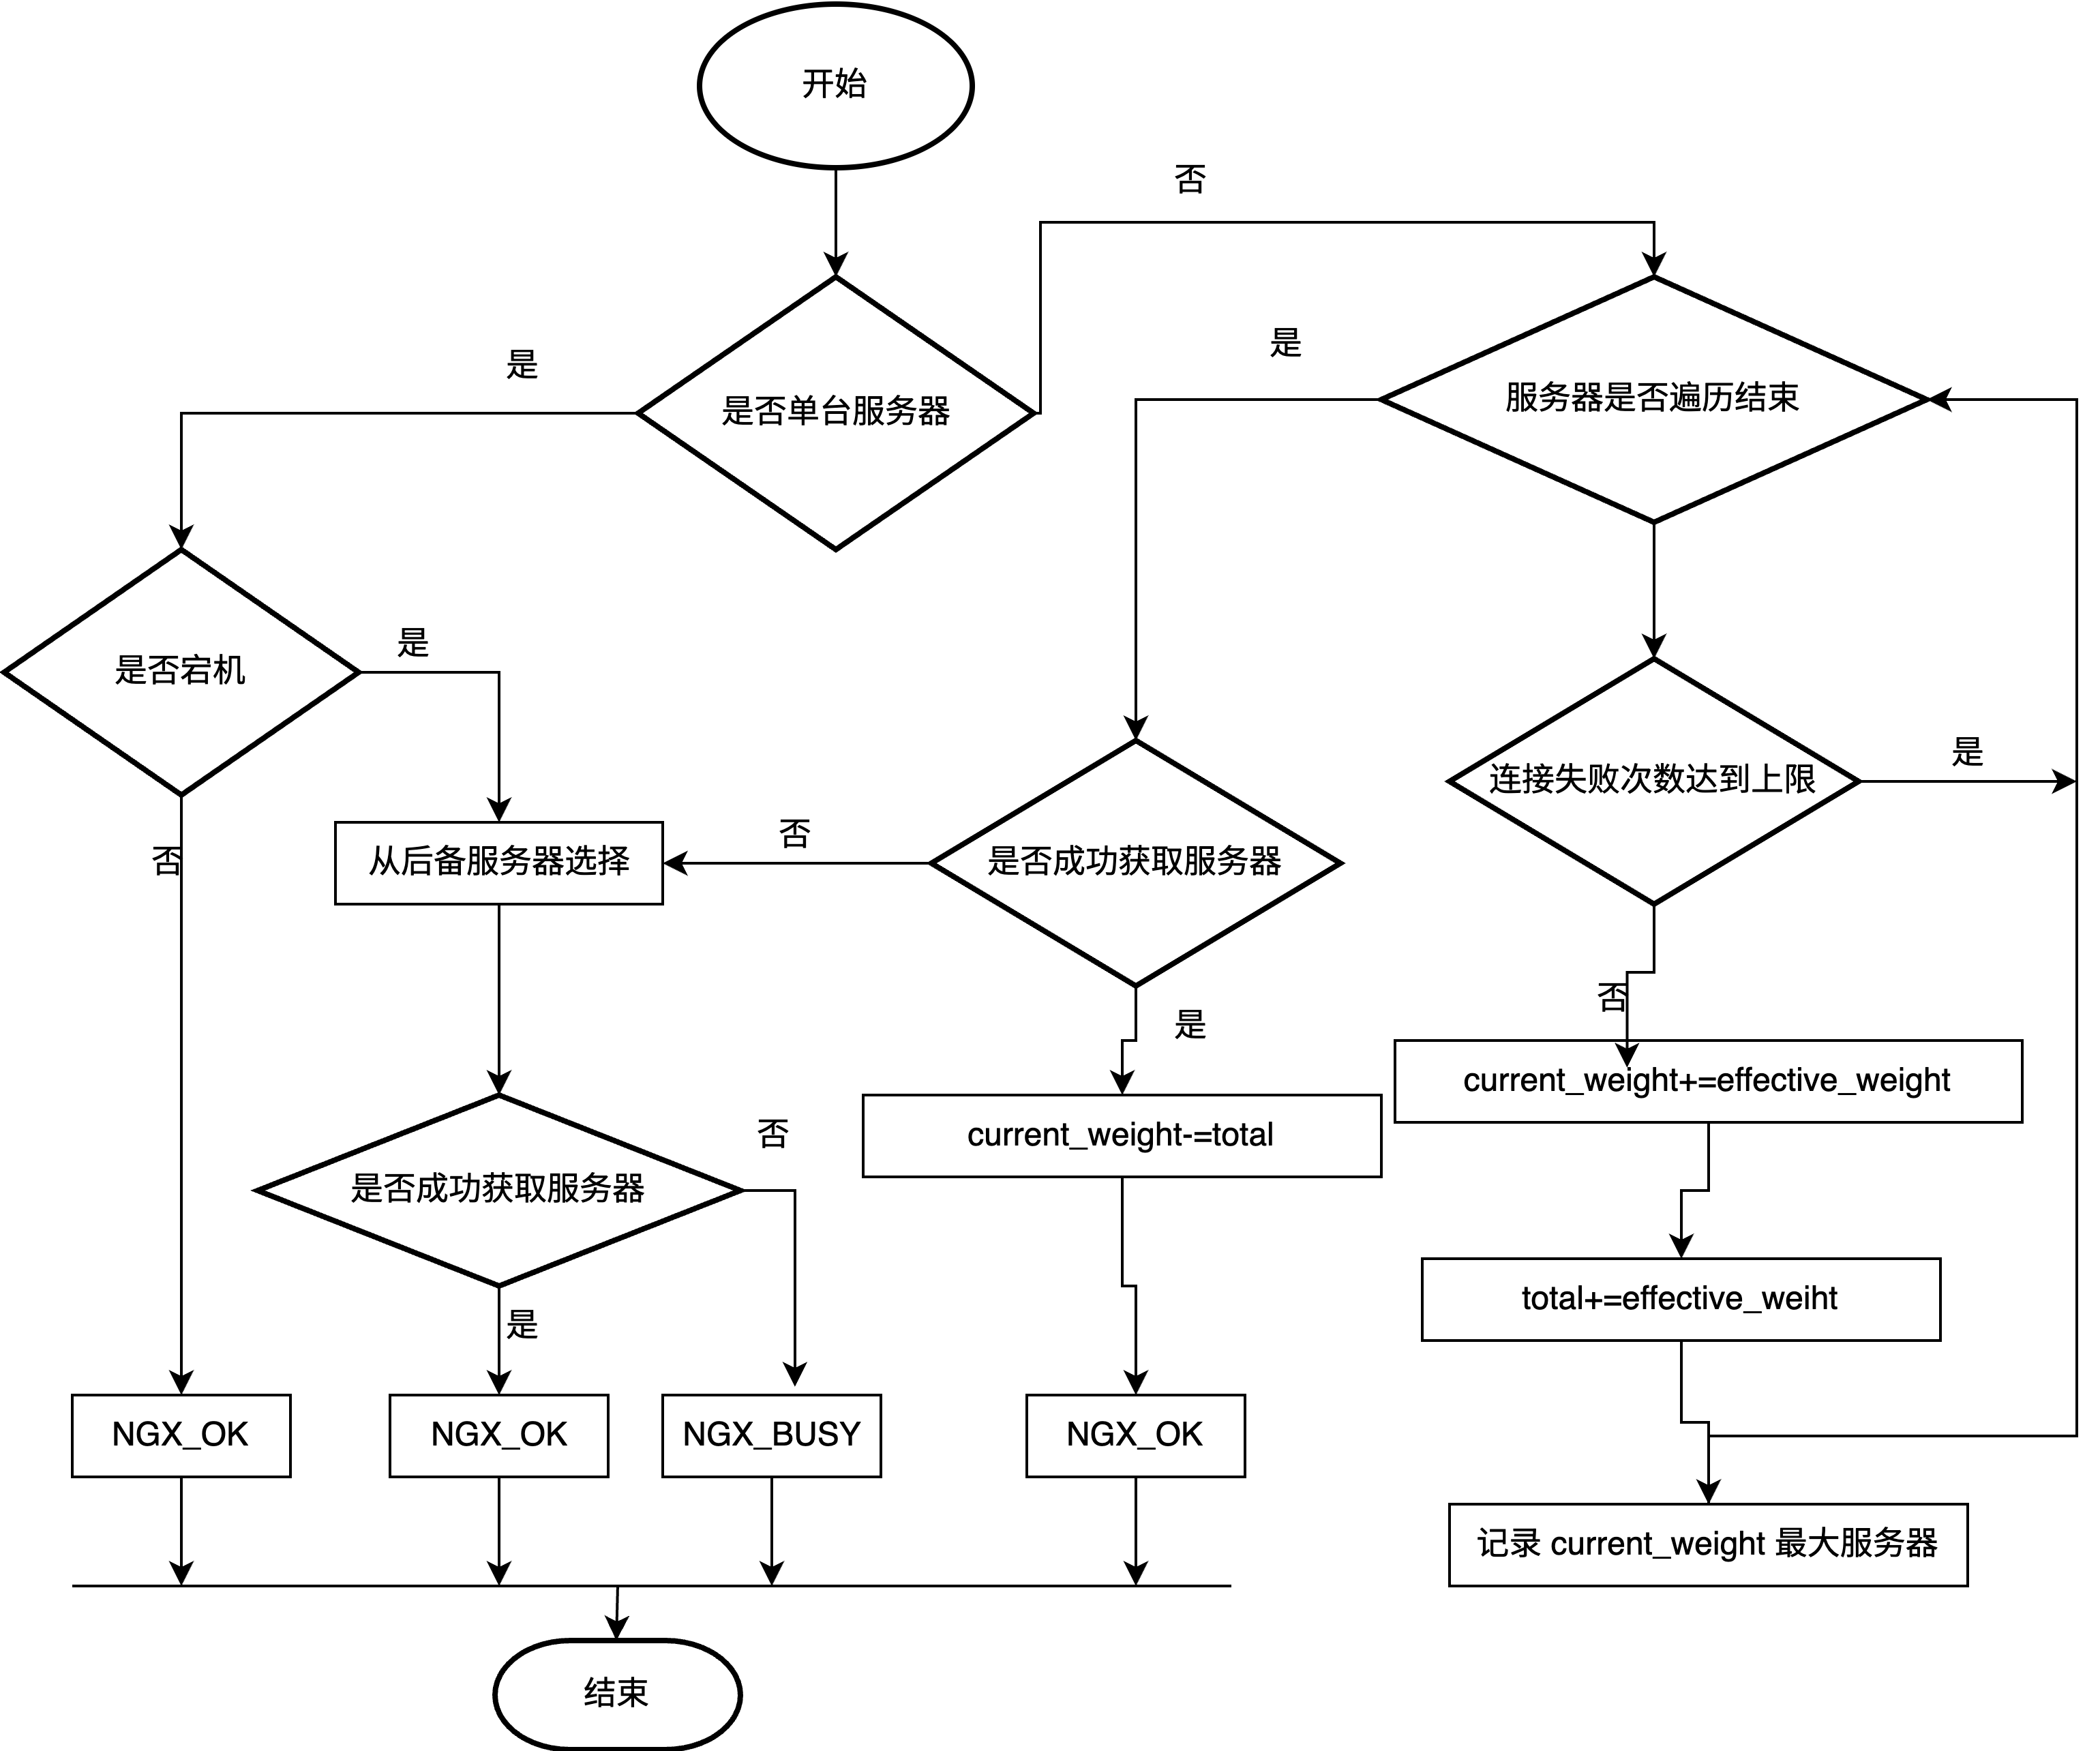
\includegraphics[width=\textwidth]{figures/round-flowchart.png}
	\caption{Nginx 加权轮询算法流程图}
	\label{weight_round}
\end{figure}

加权轮询算法,虽然考虑了上游服务器节点的不同性能差异,执行效率较高,节点选择频次相对平滑,
配置简单,但是在具体任务过程中,有些任务比较繁忙,有些任务比较轻松,这种静态的权重调节无法根据真实负载
情况进行动态调整。为了解决这个问题,诞生了动态权值的加权轮询算法,基于手机各个后台服务器节点工作时的 CPU
利用率、内存利用率、网络性能和磁盘IO等性能情况,动态的调整后端服务器节点权重\cite{谭畅2021云中心基于}。该算法在高并发
的场景下,响应时间和实际并发方面表现更好。

传统的加权轮询算法虽然在分配请求时考虑到了不同服务器节点的处理能力,通过赋予权重来实现不均等的请求分发,但在处理某些特定权重配置下,此算法可能会产生不均匀的服务实例调度序列。此现象可能导致个别实例暂时承受高强度的负载,从而使得系统面临过载甚至宕机的风险。
为了克服这一缺陷并优化负载的平滑性,研究者提出了平滑加权轮询(Smooth Weighted Round-Robin, SWRR)调度算法。相比于常规的加权轮询,SWRR算法在分发请求时更为细致地平衡了实例间的负载,旨在避免任何单一实例的瞬时过载现象。在 Nginx 中,SWRR算法通过其精巧设计的流程图,如图\ref{pinghualunxun} 所示,确保了在处理并发请求时的均衡分配,进而减少了系统宕机的风险。

\begin{figure}[htbp]
	\centering
	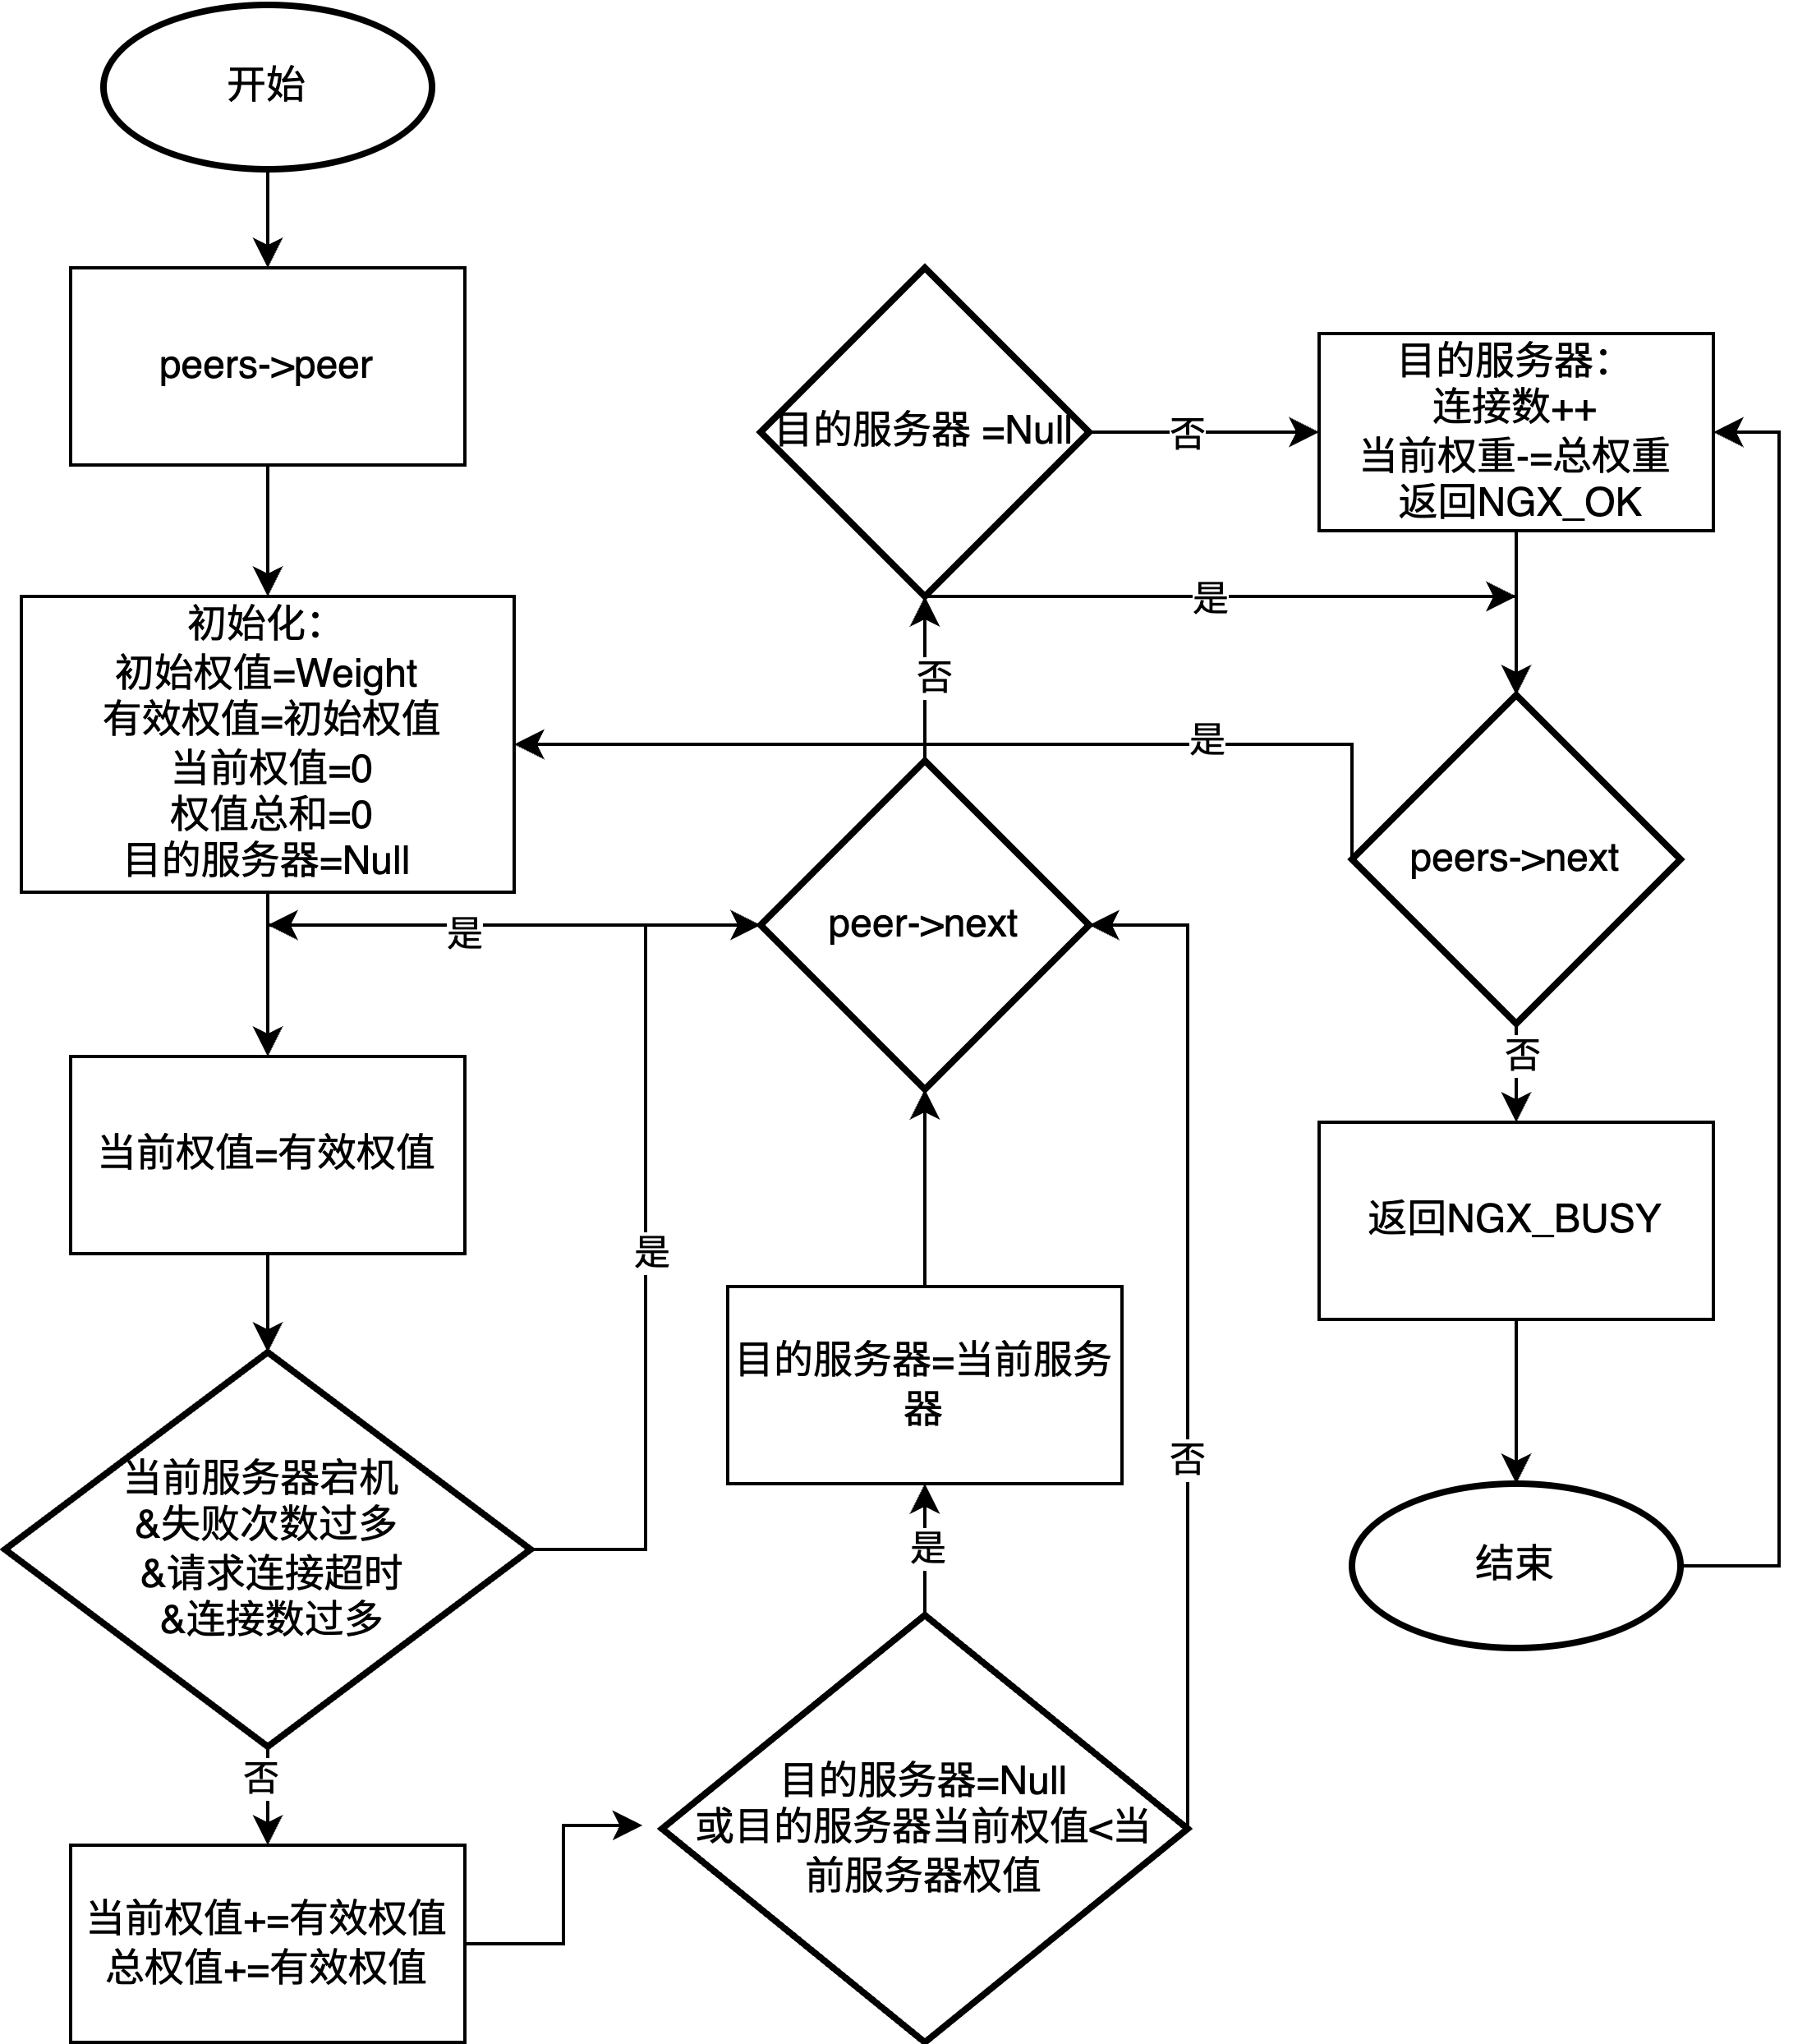
\includegraphics[width=.8\textwidth]{figures/smooth_weight.png}
	\caption{Nginx 内置平滑轮询算法流程图}
	\label{pinghualunxun}
\end{figure}

为了证明平滑性,只要证明不要一直都是连续选择那一个节点即可。假设总权重为 S,假如某个节点 i 连续选择了 t($t < x_i$) 次,只要存在下一次选择的不是节点 i,即可证明是平滑的。

假设 $t = x_i - 1$,此时第 i 个结点的当前权重为 $w_i = t \* x_i - t \* S = (x_i - 1) \* x_i - (x_i - 1) \* S$。即证明下一轮的第 1 步执行完的值 $w_i + x_i$ 不是最大。
\begin{equation}
	w_i + x_i => (x_i - 1) \* x_i - (x_i - 1) \* S + x_i =>x_i^2 - x_i \* S + S => (x_i - 1) \* (x_i - S) + x_i
\end{equation}

因为 $x_i$ 恒小于 S,所以 $x_i - S <= -1$。所以上面:$(x_i - 1) \* (x_i - S) + x_i <= (x_i - 1) \* -1 + x_i = -x_i + 1 + x_i = 1$。所以第 t 轮后,再执行完第 1 步的值 $w_i + x_i <= 1$。如果这 t 轮刚好是最开始的 t 轮,则必定存在另一个结点 j 的值为 $x_j \* t$,所以有 $w_i + x_i <= 1 < 1 \* t < x_j \* t$。所以下一轮肯定不会选中 i。

平滑加权轮询算法改善了加权轮询算法调度的缺陷,即调度序列分散的不均匀,避免了实例负载突然加重的可能,但是仍然不能动态感知每个实例的负载。若由于实例权重配置不合理,或者一些其他原因加重系统负载的情况,平滑加权轮询都无法实现每个实例的负载均衡,这时就需要有状态的调度算法来完成。由此本文在该算法基础上进行了相关调整,首先采集后台各个节点指标数据,包括 CPU、内存、网络带宽以及磁盘I/O指标数据,并对采集到的数据惊醒相关处理,通过这些数据来确定不同节点的初始权重,反应不同节点的初始性能差异。并持续周期性的收集综合负载指标,使用训练好的模型预测剩余性能,并根据该性能调整节点权重。同时为了防止初期无法得到有效的服务器负载均衡后的有效数据,将会使用默认的平滑加权算法来得到初期数据,经过一定周期,将收集到的负载均衡数据整理并使用预测模型进行预测,并根据预测的数据进行初始权重的调整和优化。

\section{改进的负载均衡算法的提出}
本次改进后的动态加权轮询算法涵盖了四个主要模块,分别为服务器负载信息收集模块,服务器信息处理模块,Nginx 动态加权轮询模块以及周期性预测模块。这些模块相互配合,共同实现了算法的全面功能:

(1) 服务器负载信息收集模块:此模块持续运行在集群的各个节点上,周期性地收集节点的负载数据,如访问次数、CPU、内存、网络带宽和磁盘I/O等指标,并将这些数据存储到 Memcached 中。
(2)服务器信息处理模块:在 Nginx 负载均衡服务器上运行,该模块从 Memcached 中提取各节点的负载数据,并综合这些信息来评估各个节点的整体负载情况。根据预设的阈值 M 和 N 进行比较,以判断节点的负载是否处于正常范围内。若节点负载异常,模块将调整该节点的权重,并更新至 Memcached。
(3)周期性预测模块:基于网站访问量及综合负载指标,周期性地进行负载预测,并据此调整阈值 M 和 N,以优化负载平衡效果。
(4)Nginx 动态加权轮询模块:从 Memcached 中获取节点的最新权重信息,并依据改进的算法逻辑,选择合适的节点处理新的任务请求。

系统的整体结构设计旨在实现高效、灵活的负载均衡,以优化资源利用率和响应性能。其框架如下图所示(请见图\ref{total_structure_flow})。

\begin{figure}[htbp]
	\centering
	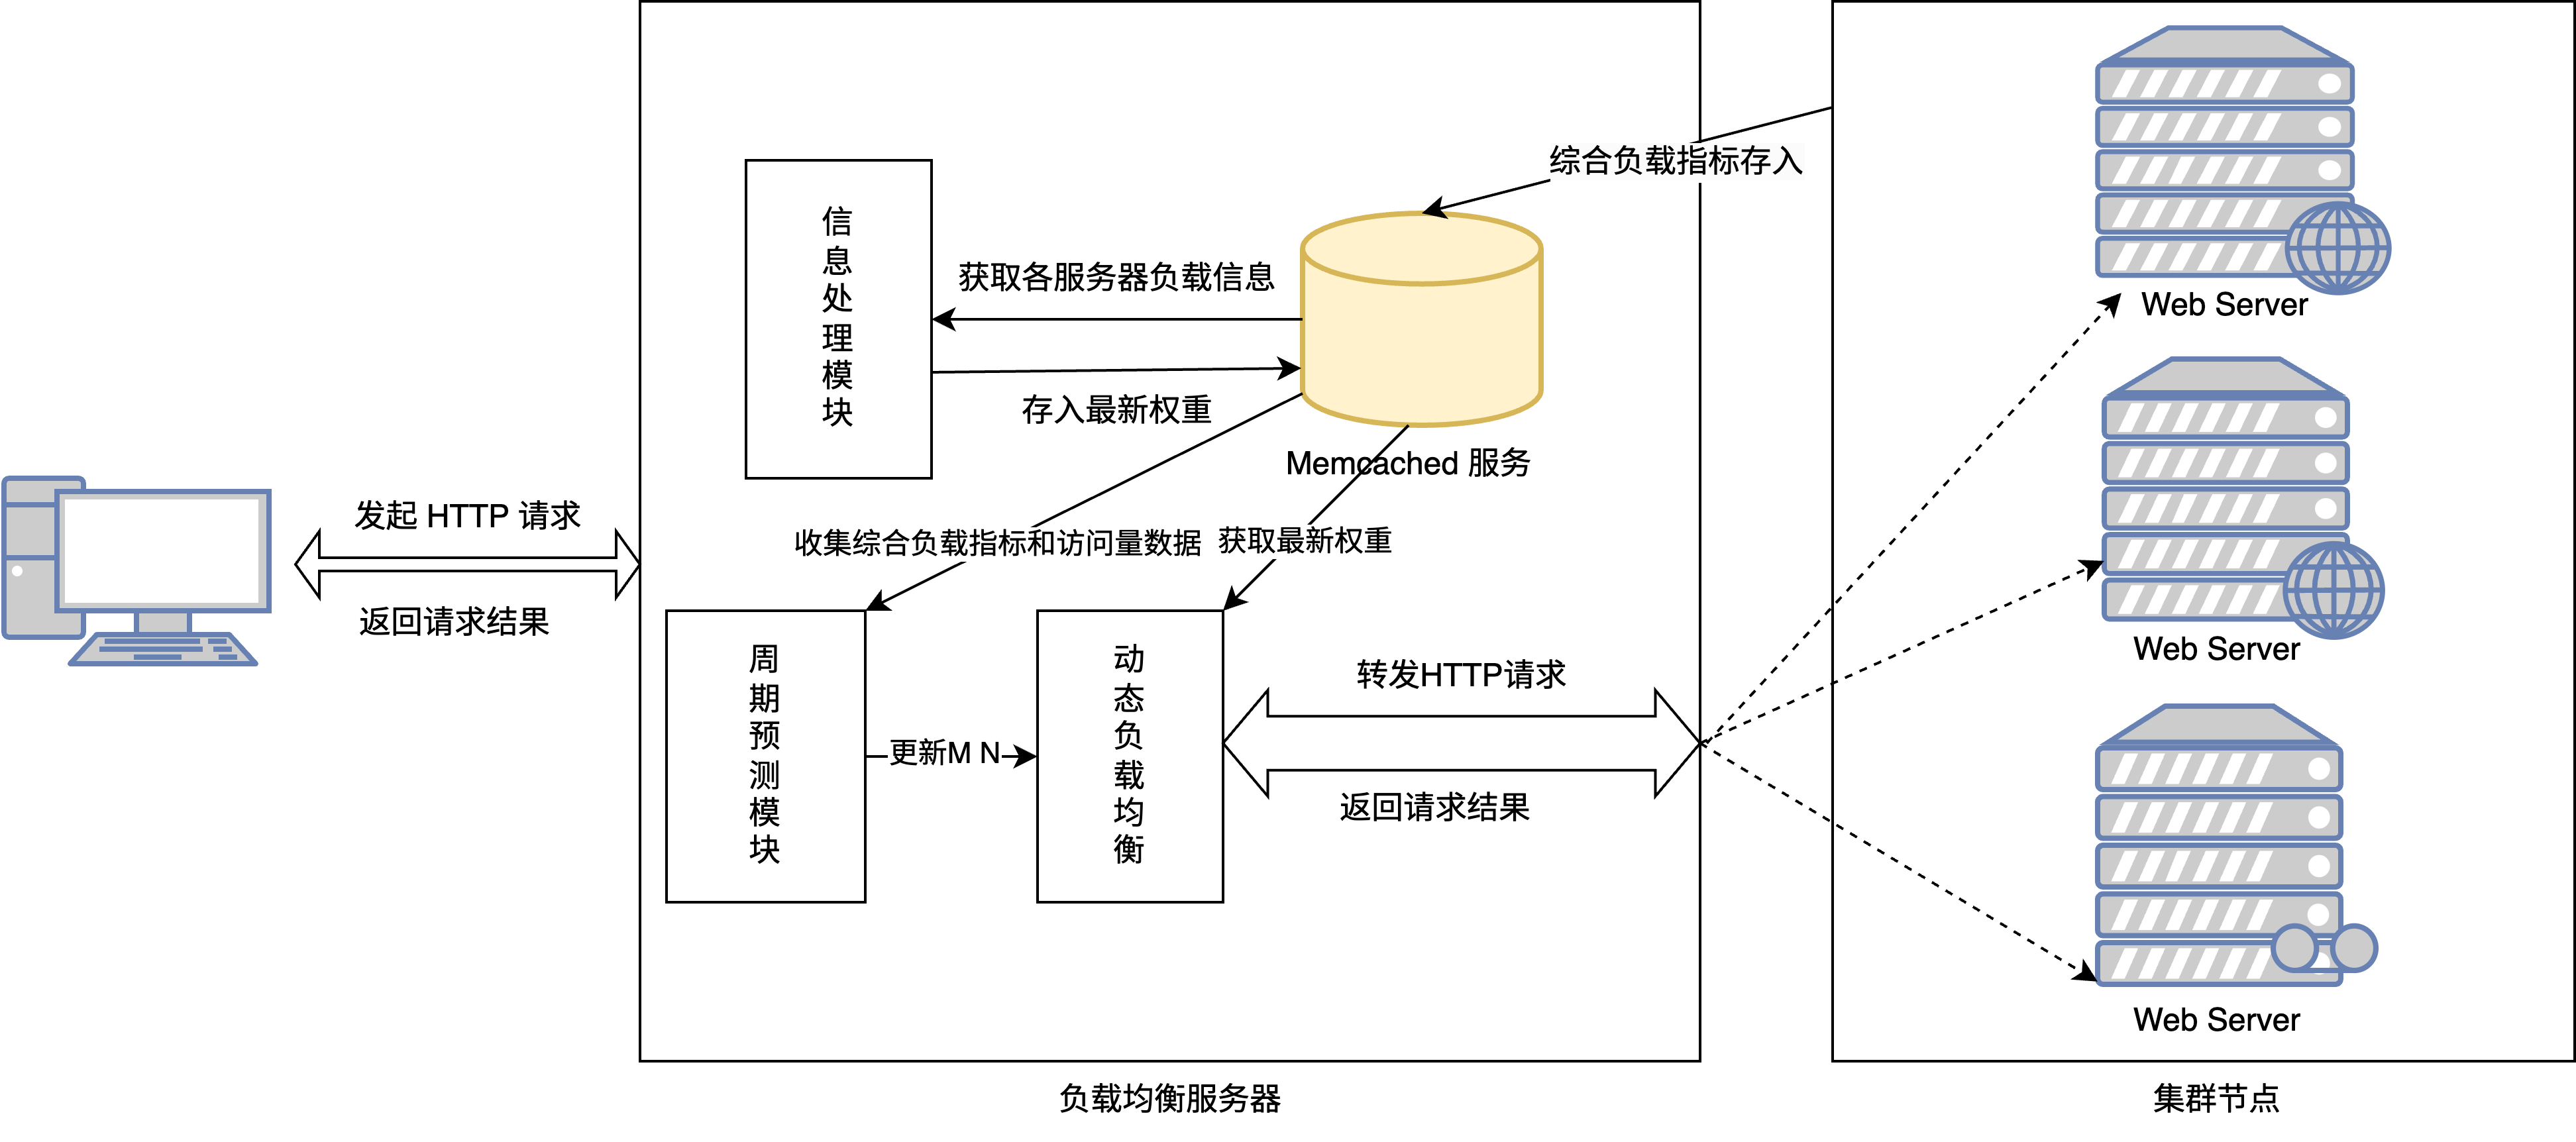
\includegraphics[width=\textwidth]{figures/landbalance_module.png}
	\caption{总体结构图}
	\label{total_structure_flow}
\end{figure}

当客户端用户发起 HTTP 请求时,该请求被发送至 Nginx 服务器。Nginx 服务器根据其配置的负载均衡策略选择集群中的一台服务器节点,进而将客户端请求转发至该节点。
所选节点随后处理这个请求,并将处理结果回传给 Nginx 服务器。Nginx 再将这些数据回送给客户端,客户端接收到这些响应数据后进行相应的处理,并在网页上显示结果。
在此流程中,采用了改进后的平滑动态加权轮询算法,以优化请求的分发和处理效率,确保系统负载均衡。该算法的详细流程展示在下图中(详见图\ref{new_smoth_weight_balance})。

\begin{figure}[htbp]
	\centering
	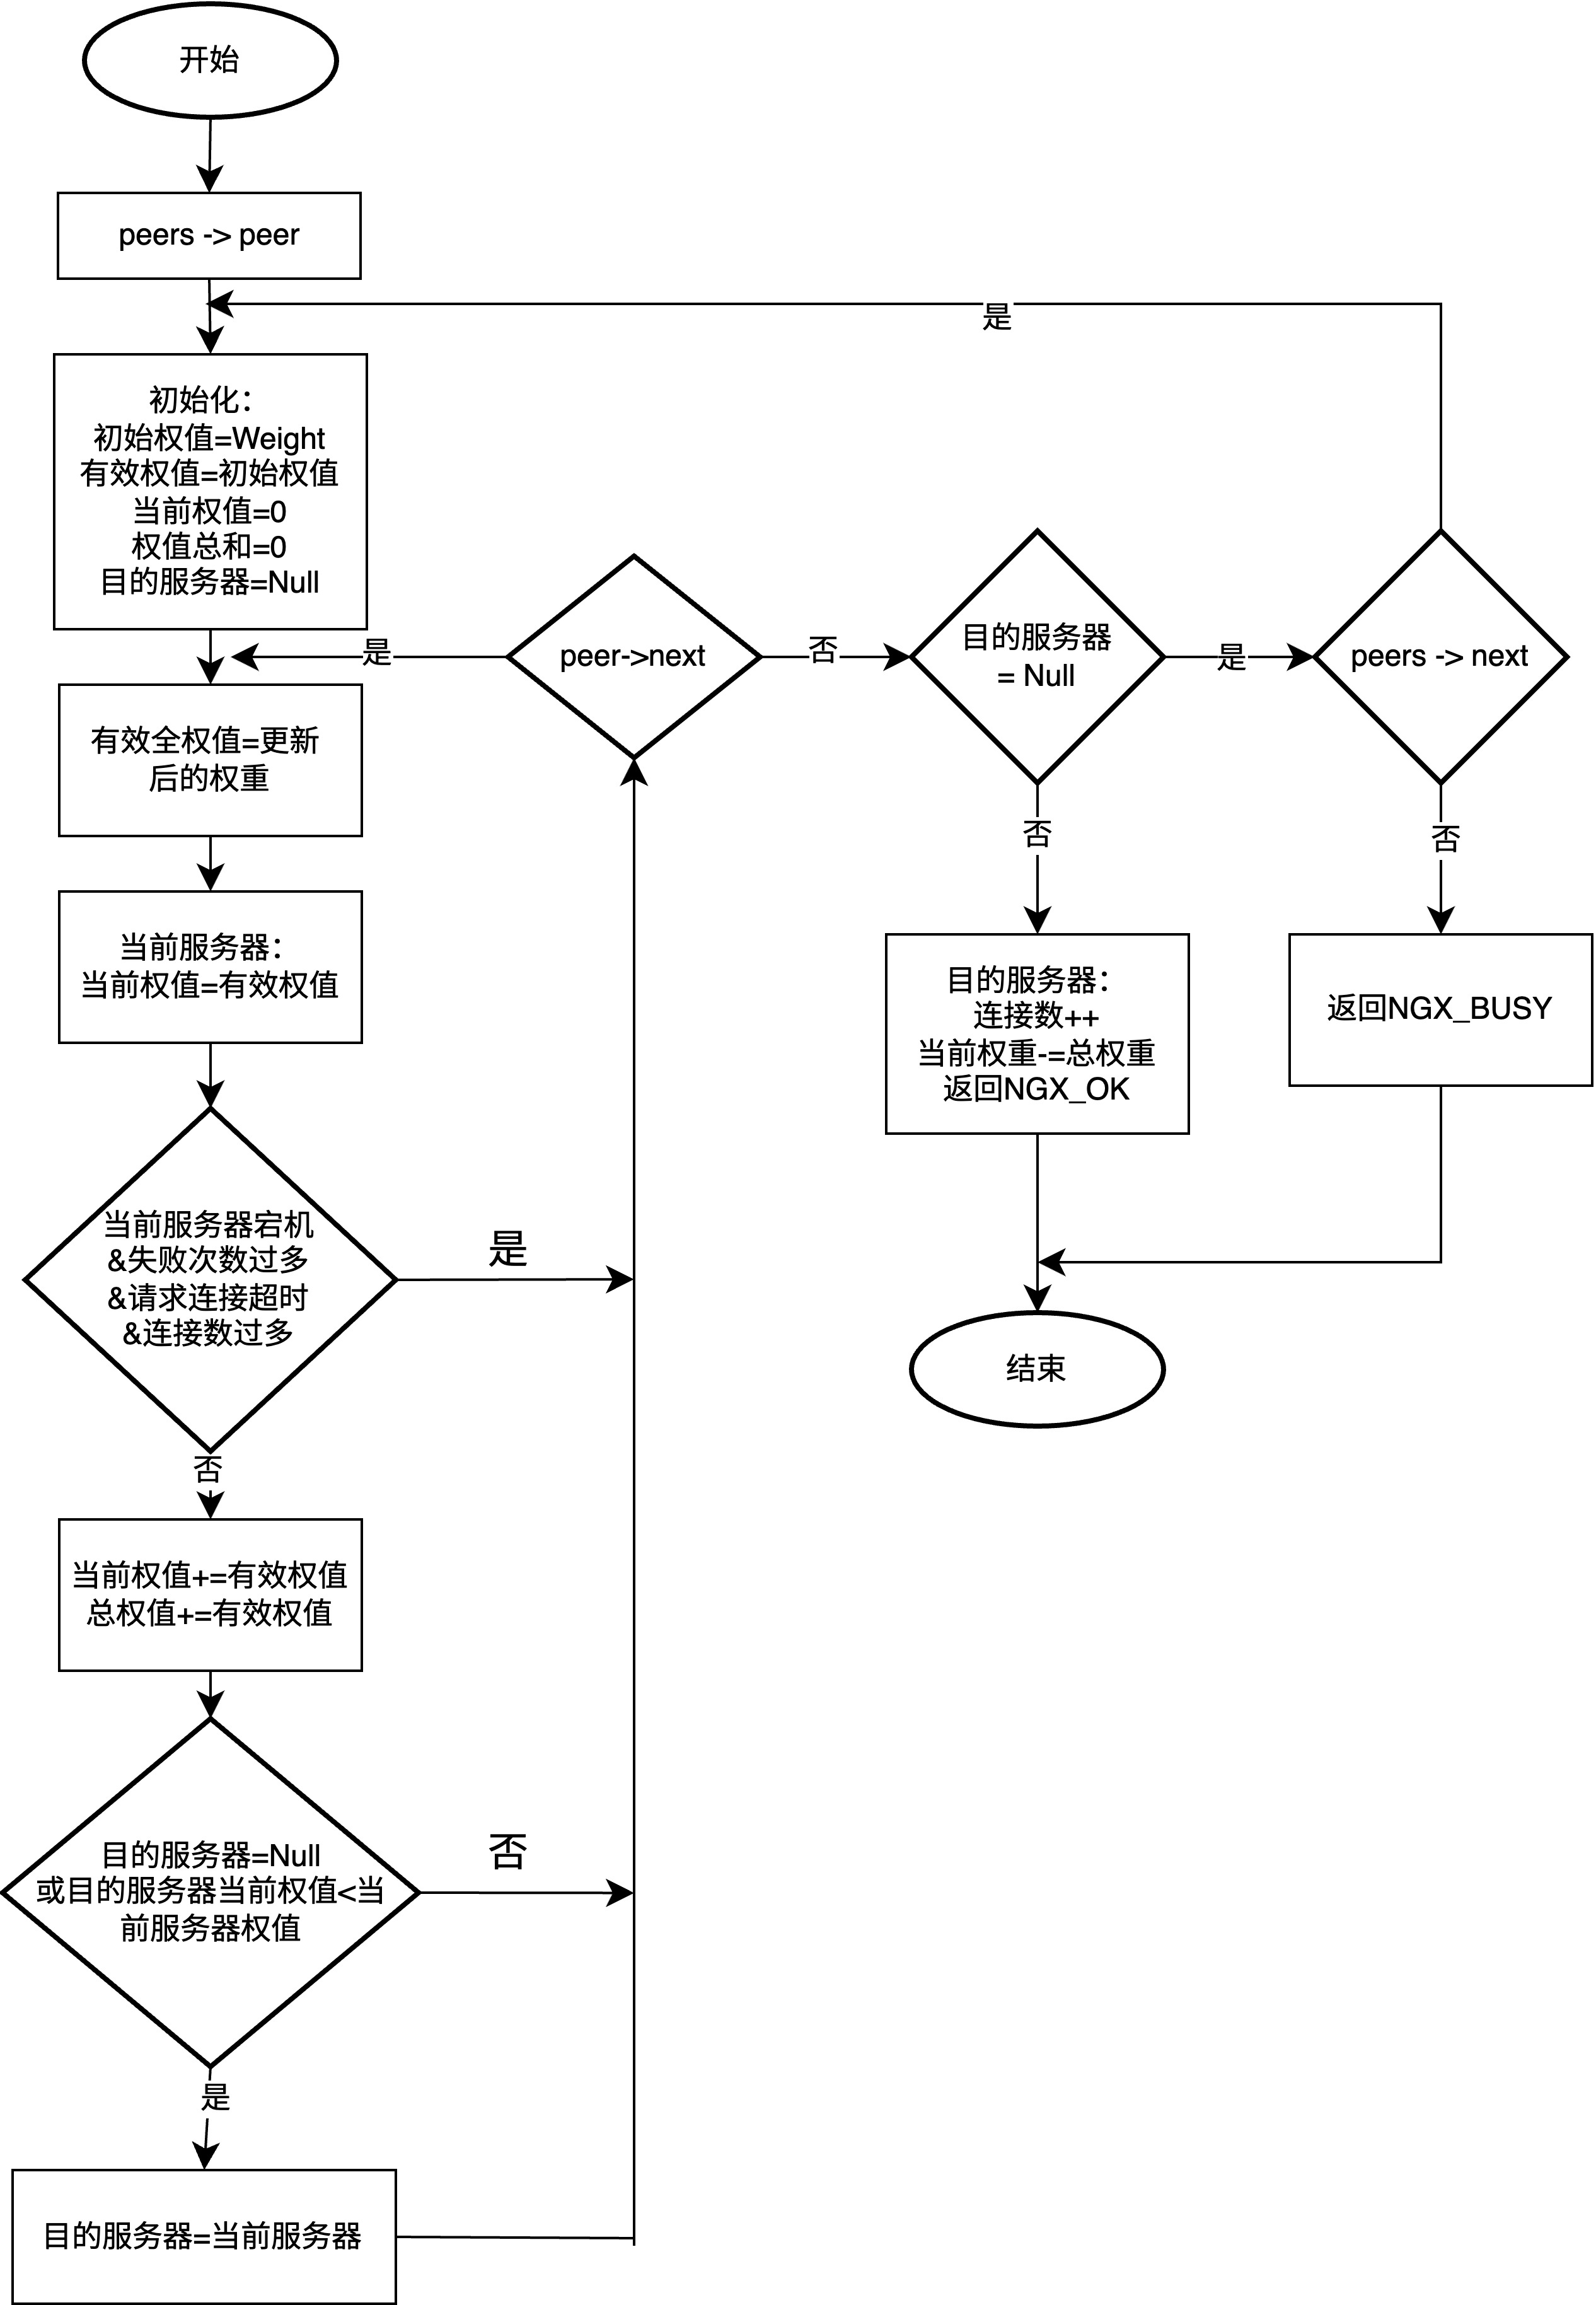
\includegraphics[width=\textwidth]{figures/new_smoth_weight_balance.jpg}
	\caption{改进后的平滑加权轮询算法流程图}
	\label{new_smoth_weight_balance}
\end{figure}

改进后的算法由两个阶段构成:第一个阶段是没有预测负载指标的情况,第二个阶段则是已有预测负载指标的情况。一开始,由于缺少适当的数据,算法通过周期性处理模块分析当前服务的访问量和服务器负载状况,此时采用常规的平滑加权轮询算法执行初始任务分配。
在这个阶段,服务器负载信息收集模块负责收集每个后端节点目前的 CPU、IO、内存以及网络带宽使用率。

紧接着,将每个节点的负载数据送至服务器信息处理模块和周期性预测模块进行数学分析,通过特定公式计算得到每个节点的总体负载情况。
根据设定的阈值来判断节点是否平衡,若不平衡则更新其权重数据。一旦节点权重分析完成,Nginx 的平滑加权轮询模块即可获取更新后的权重信息。

随后进行服务器配置及权重的初始化操作,初始化完成后,通过 nginx\_http\_upstream\_get\_dynlb\_select\_peer
函数选出所有可用上游服务器中 current\_weight 最高的服务器来处理请求。
若所有节点都不符合条件,则默认回落到 Nginx 自身的轮询算法。请求处理完毕之后,调用 ngx\_http\_upstream\_free\_dynlb\_select\_peer 以释放系统资源,以此提升算法效率。
第二阶段基本与第一阶段相似,但是在阈值设定和初始权重调整方面会有所区别,加入了周期性预测后的访问量权重考虑和综合负载指标权重预测的考虑。

\section{负载均衡算法的优化}
通过第三章、第四章预测访问量的算法和剩余性能深度学习卷积神经网络的研究,有效的证明了算法的有效性和深度学习网络的优秀性能。通过对访问量的预测能够有效的在根据不同时间内分配合适的任务量,优化集群内的节点效率,有效降低集群的资金输入。通过时间卷积网络则可以很好的提取到不同时间段蕴藏的信息,同时得到了节点未来的负载情况,使得负载均衡器有效的分配合适的任务给合适的集群节点。
但是对于初期没有负载数据和访问量数据的问题,也需要值得重视,本节既是为了研究初期负载算法的优化。

第四章中通过主成分分析法分析了在已有数据情况下的公式(1.1)的权重参数,但是在没有数据之前仍然需要通过一定的分析得出一个较为合理的权重和综合负载情况的阈值。通过对不同论文的研究\cite{吴文辉2013编程计算层次分析法},本文选择了层次分析法来进行初期的权重参数的计算。

首先,需要构建出层次分析模型。将综合负载指标作为目标层,CPU、内存、网络带宽以及磁盘IO利用率指标作为准则层,层次分析模型结构如下图\ref{Layered_Analysis}所示。

\begin{figure}[htbp]
	\centering
	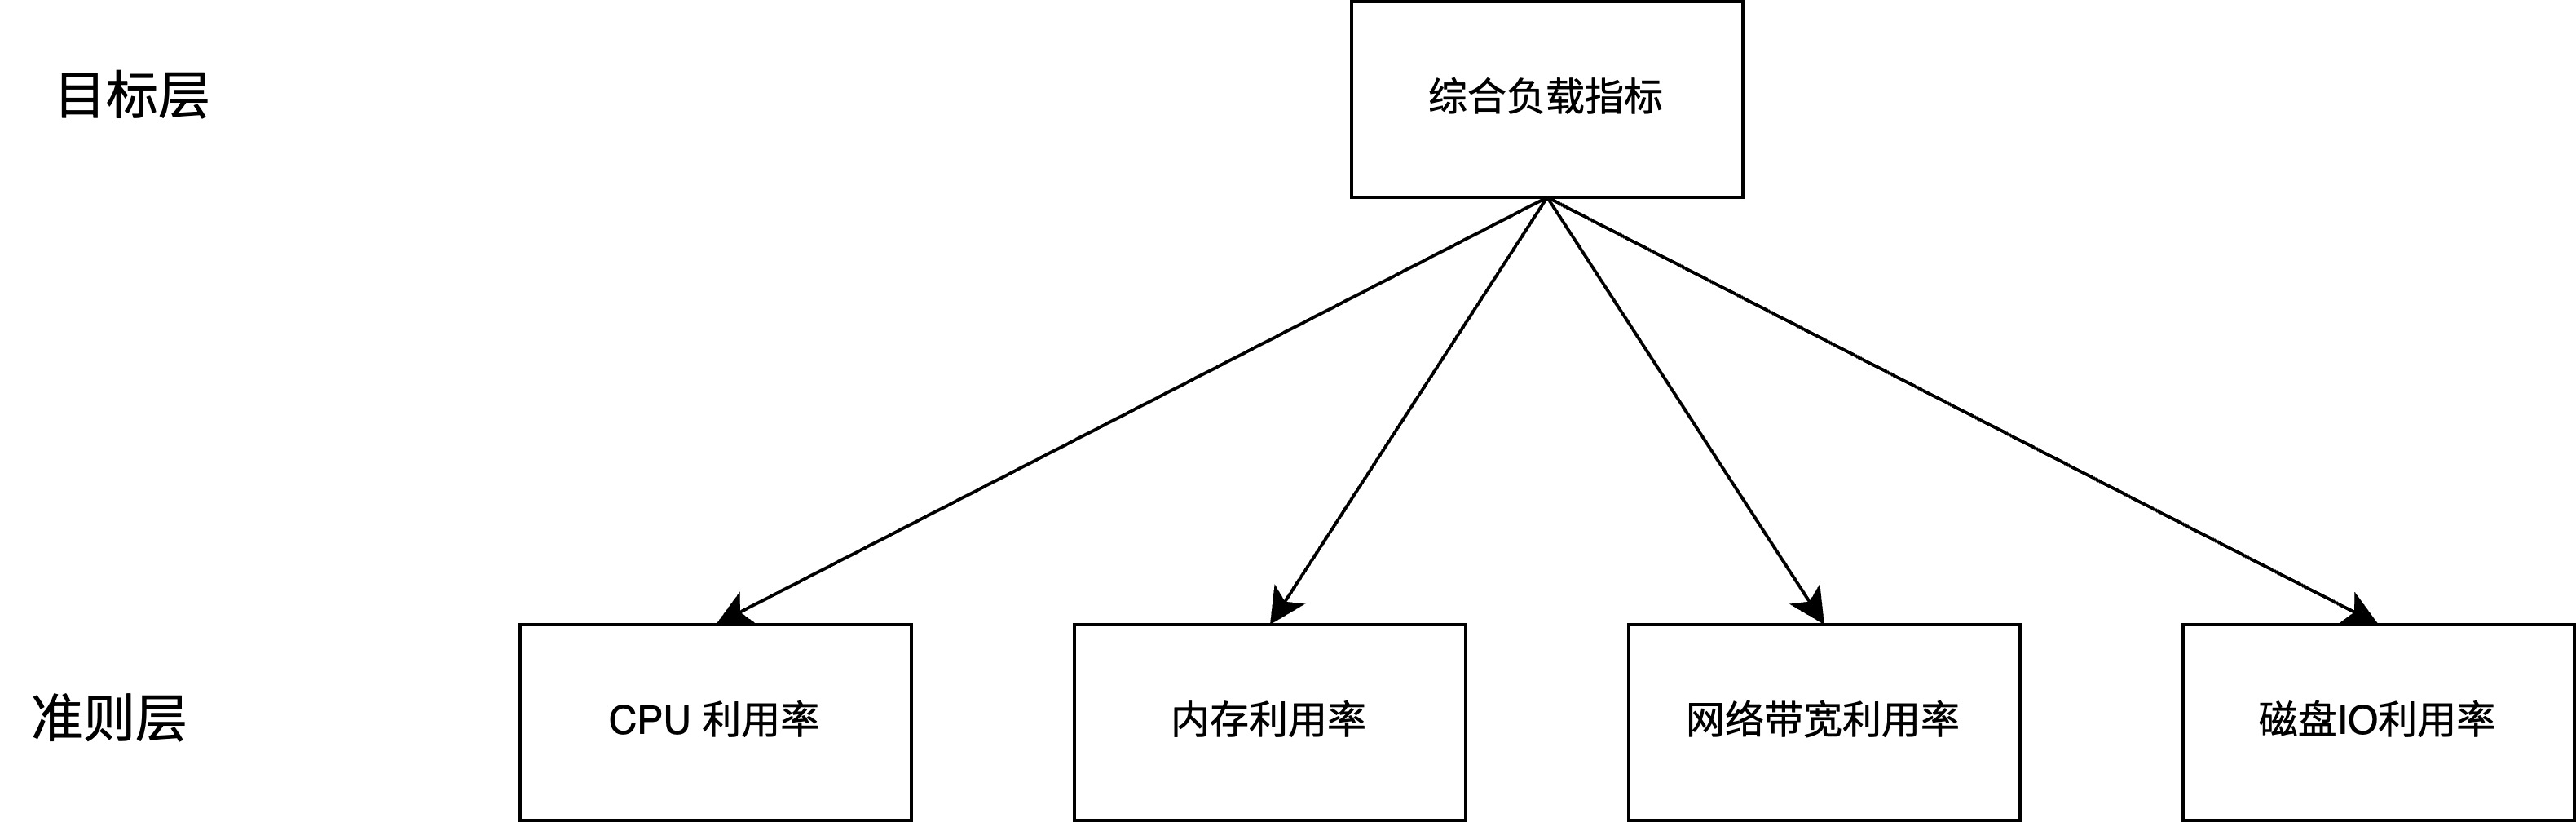
\includegraphics[width=\textwidth]{figures/Layered_Analysis.jpg}
	\caption{综合负载层次分析模型}
	\label{Layered_Analysis}
\end{figure}

采用 “1-9” 标度法,结合服务器测试情况构建判断矩阵。根据论文得知,CPU、内存利用率较高,而网络带宽与磁盘IO利用率相对较低\cite{吴陈2020基于Nginx的服务器集群负载均衡策略的研究与改进}。服务器对资源消耗标度表如下。

% \usepackage{tabularray}
\begin{longtblr}[
	caption = {服务器对资源消耗情况},
	]{
	width = \linewidth,
	colspec = {Q[146]Q[331]Q[331]Q[113]Q[79]},
	vline{2-5} = {-}{},
	hline{1,6} = {-}{0.08em},
			hline{2} = {-}{},
		}
	Q   & CPU           & Mem           & Net & IO \\
	CPU & 1             & 1             & 3   & 3  \\
	Mem & 1             & 1             & 3   & 3  \\
	Net & $\frac{1}{3}$ & $\frac{1}{3}$ & 1   & 1  \\
	IO  & $\frac{1}{3}$ & $\frac{1}{3}$ & 1   & 1
\end{longtblr}

于是,得到了判断矩阵:
\begin{equation}
	Q = \begin{bmatrix}
		1   & 1   & 3 & 3 \\
		1   & 1   & 3 & 3 \\
		1/3 & 1/3 & 1 & 1 \\
		1/3 & 1/3 & 1 & 1
	\end{bmatrix}
\end{equation}

按照层次分析法的要求,得到了判断矩阵,通过合积法计算其近似特征向量。首先将矩阵(5.2)按照公式(5.3),再按列相加再做归一化,归一化的元素按行相加得到的结果处理后如下表所示。
\begin{equation}
	q_{ij}= \frac{q_{ij}}{\sum_{i=1}^{n}q_{ij} }(i,j = 1,2,\dots ,n)
\end{equation}

% \usepackage{tabularray}
\begin{longtblr}[
	caption = {对比表},
	]{
	width = \linewidth,
	colspec = {Q[167]Q[179]Q[179]Q[179]Q[179]Q[113]},
	vlines,
	hline{1,6} = {-}{0.08em},
			hline{2} = {-}{},
		}
	Q   & CPU   & Mem   & Net   & IO    & ∑   \\
	CPU & 0.375 & 0.375 & 0.375 & 0.375 & 1.5 \\
	Mem & 0.375 & 0.375 & 0.375 & 0.375 & 1.5 \\
	Net & 0.125 & 0.125 & 0.125 & 0.125 & 0.5 \\
	IO  & 0.125 & 0.125 & 0.125 & 0.125 & 0.5
\end{longtblr}

对上表自左向右最后一列元素进行归一化处理之后,即可得到特征向量 $M'=(M_1, M_2, M_3,\dots,M_n)^\mathbf{T}$的近似特征向量 $M'$。
\[
	M' = (0.375, 0.375, 0.125, 0.125)
\]
于是初始阶段的权重已经确定,则初期阶段综合负载决策函数为:
\begin{equation}
	X = 0.375\times(CPU) + 0.375 \times (Mem) + 0.125 \times (Net) + 0.125\times(IO)
\end{equation}

当节点的资源使用率达到了系统的瓶颈时,节点处理任务请求的效率就会明显下降,那么负载均衡器分配给节点的权重值就会减少。
通过表(2.2)可知,当节点的资源利用率评价为坏的时候,则可以认为此时节点负载过高。
在初期阶段,此时总体剩余利用率可以通过公式(5.4)计算得到,在使用了周期性预测模块阶段则通过(4.4)计算得到,将该值设为 M。
M 是判断节点负载是否平衡的条件,当 $X \ge M$  时,判断节点为高负载状态,则可以取阈值$N = 1 - M / 2$。

信息采集周期 $\mathbf{T}$ ,在负载信息收集模块和周期性预测模块中起着关键作用。如果采集周期设置过短,在提高数据收集实时性的同时,可能会由于频繁的操作消耗过多系统资源。相反,如果采集周期过长,有可能导致负载均衡服务中节点的权重参数更新滞后,从而影响整体系统的响应性和效率。因此,正确地确定采集周期 $\mathbf{T}$ 并非一件简单的任务,而应通过定量的方法进行科学地评估和测试。
本研究建议利用压力测试工具如siege对不同的采集周期 $\mathbf{T}$ 进行实验对比,以便找出一个既能确保系统资源有效利用,又能保持权重参数及时更新的最优周期。

Siege 是一款广受欢迎的开源压力测试工具,其主要目标是评估 WEB 应用在高负载条件下的性能表现。
Siege 能够根据预设置的配置,模拟多用户并发访问网站,同时记录每一个用户请求的响应时间。
这些测试可以在特定的并发访问量下重复执行,以生成一组全面且可靠的性能数据。针对不同业务需求,Siege 允许用户自定义测试并发量,并选择针对存储在指定文本文件中的不同链接进行访问,以模拟真实世界的负载环境。具体的并发量和任务类型取决于应用的业务场景和性能需求,以下是一些推荐的配置方式。

% \usepackage{tabularray}
\begin{longtblr}[
	caption = {企业与任务类型},
	]{
	width = \linewidth,
	colspec = {Q[323]Q[408]Q[146]},
	vline{3} = {-}{},
	hline{1,6} = {-}{0.08em},
			hline{2} = {-}{},
		}
	企业类型  & 并发量          & 任务 \\
	小型企业  & 500-1000     & 文本 \\
	中型企业  & 1000-5000    & 图片 \\
	大型企业  & 10000-100000 & 音频 \\
	超大型企业 & 100000-      & 视频
\end{longtblr}
siege 的测试命令如下。
\noindent \begin{lstlisting}[caption={siege 的测试命令}]
siege -c 并发量 -r 重复次数 -f url.txt
\end{lstlisting}

其中url.txt 则是指定的任务类型,具体类型如下。
\noindent \begin{lstlisting}[caption={url.txt 请求任务类型}]
http://192.168.66.166/xx.jpg
http://192.168.66.166/xx.html
http://192.168.66.166/06.mpv
http://192.168.66.166/06.mp4
\end{lstlisting}

通过siege的测试可以得到不同周期 $T$ 下Nginx 的负载程度,通过对Nginx负载程度的定量分析,可以得到当前业务下最适合的周期 $T$。同时在周期预测阶段则可以选择每小时,每天,每月,每年作为整个周期进行拟合和预测。

在改进的动态负载均衡策略中,有两个重要部分,其一是使用合适的周期来收集各个服务器节点的剩余性能,并保存在 Memcached 服务中。Memcached 是一个分布式的告诉缓存系统,对于频繁获取负载信息的操作很有利,保证了收集数据的实时性,控制了资源的消耗。
其二,如果负载均衡器判断了集群某些节点负载不均衡后,如何调整各个节点的权重。

在本算法中,使用阻塞控制的思想来对权重进行调整。
拥塞控制是作用于网络的,它是防止过多的数据注入到网络中,避免出现网络负载过大的情况;常用的方法就是:( 1 )慢开始、拥塞避免( 2 )快重传、快恢复。本改进算法使用了,快重传,和快恢复算法。
常见的改进的动态负载均衡方法使用的是TCP Tahoe 算法,但是现在已经遭到抛弃。所以本算法使用的是 TCP Reno 算法。

快速重传协议要求,在接收到一个乱序的报文段后,接收方应立即发送重复确认,而不是等待其自身发送数据时再附带确认。具体来说,一旦发送方连续收到三个重复确认,便应立即重传还未被接收方收到的报文段,无需等待预设的重传定时器超时。

配合快速重传,还有一种被称为"快速恢复”的算法。当发送方连续收到三个重复确认时,便会执行“乘法减小”算法,将慢启动门限(ssthresh)减半,以预防网络拥塞。
不过,在此之后,系统并未执行慢启动算法。这是因为,如果网络真的发生了拥塞,发送方就无法收到多个连续的重复确认。
因此,发送方在此刻认为网络可能并未发生拥塞。于是,系统并未执行慢启动算法,而是将拥塞窗口(cwnd)设置为慢启动门限减半后的值,然后执行拥塞避免算法,使拥塞窗口缓慢增大。
下方的图表(图\ref{tcp_reno})详细展示了拥塞控制窗口和传输轮次之间的对应关系,以及改进之后的 TCP Reno 算法的具体变化。

\begin{figure}[htbp]
	\centering
	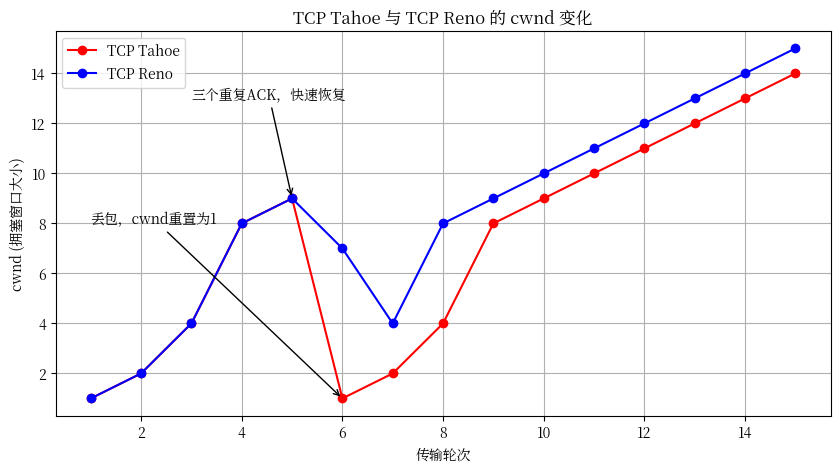
\includegraphics[width=\textwidth]{figures/tcp_reno.png}
	\caption{TCP Reno 的 cwnd 变化}
	\label{tcp_reno}
\end{figure}

TCP Reno 在 Tahoe 的基础上增加了快速恢复机制即快重传机制。在 Reno 中,当收到三个重复的 ACK 时(表示一个单一的数据包丢失),它不会像 Tahoe 那样直接进入慢启动阶段,而是进入快速恢复阶段。在这个阶段,它将阈值设为当前 cwnd 的一半,并将 cwnd 设置为新阈值加3个段的大小,然后进行拥塞避免算法。如果又出现超时,则会和 Tahoe 一样,将 cwnd 设为1,重新开始慢启动过程。Reno 的这种机制可以在某些丢包情况下避免 cwnd 的大幅度减少,使得网络能够更快地恢复到有效的传输状态。从而使的负载均衡节点更有效的调整节点的权重

根据这种思想,本文想去了服务器节点的综合负载指标这一指标作为判断负载时的条件,并设置一个阈值 $N$ 作为改进的动态轮询算法的权重调整门限,
值 $X$ 判断节点是否负载均衡的条件。传统算法中,根据服务器信息处理模块收集到的信息来进行判断具有滞后性,
因此本文通过周期性预测算法的加入,通过对综合负载指标进行预测来作为参考标准。
首先,在初期阶段,需要使用公式(5.4)的层次分析法的权重公式对参考指标进行计算,按照默认的平滑加权轮询算法进行负载均衡;
在周期性预测阶段,周期性预测模块通过使用存储在 Memcached 服务中的一段时间的综合负载指标进行预测,获取所有节点下一时间段的综合负载情况。
若判断存在某一个服务器节点下一时间会变成高负载状态,则将下一时刻判断为负载不均衡的节点进行权重调整,
调整方式为$W_j = 1000 \times X_{j} / \sum U_{i}$,$\sum U_{i}$ 表示下一时刻所有负载不均衡节点综合负载指标的和,
$W_j$为第 $j$ 个且被判断为下一时刻负载不均衡的节点,并将节点的权重信息存入 Memcached 服务。
对于高负载节点权重,将其调整为 $W_{new} = 1000 \times W_{j} / 2^{n}$ ,$n$ 为权重调整次数,直至节点到达负载均衡(快速回复)。
监控高负载节点的负载状况持续进行。当该服务器节点的综合指标, $X < N$ 且当前权重值小于初始权重值时,
节点的权重将被调整为 $W_{new} = 1000 \times W_{j} + 2^n$,其中 $n$ 是调整次数。
若权重增长值在此过程中等于初始权重值,则会调节权重增长的速率。单服务器节点的综合负载指标 $X \ge N$ 且当前权重小于初始权重值,则将停止该节点的指数型增长,并转为线性增长。
此时, $W_{new} = 1000 \times W_{j} + 2^k + n$, 其中 $k$ 为停止指数增长此刻权重调整的次数。
如果在此过程中权重达到初始权重值,权重增长将停止。然而,如果该节点在下一时期再次被判断为高负载状况,则将再次调整权重。
在节点权重信息调整过程中,权重值会持续更新并记录在 Memcached 中。高负载节点权重调整的流程图如图\ref{contral_weight}所示。

\begin{figure}[htbp]
	\centering
	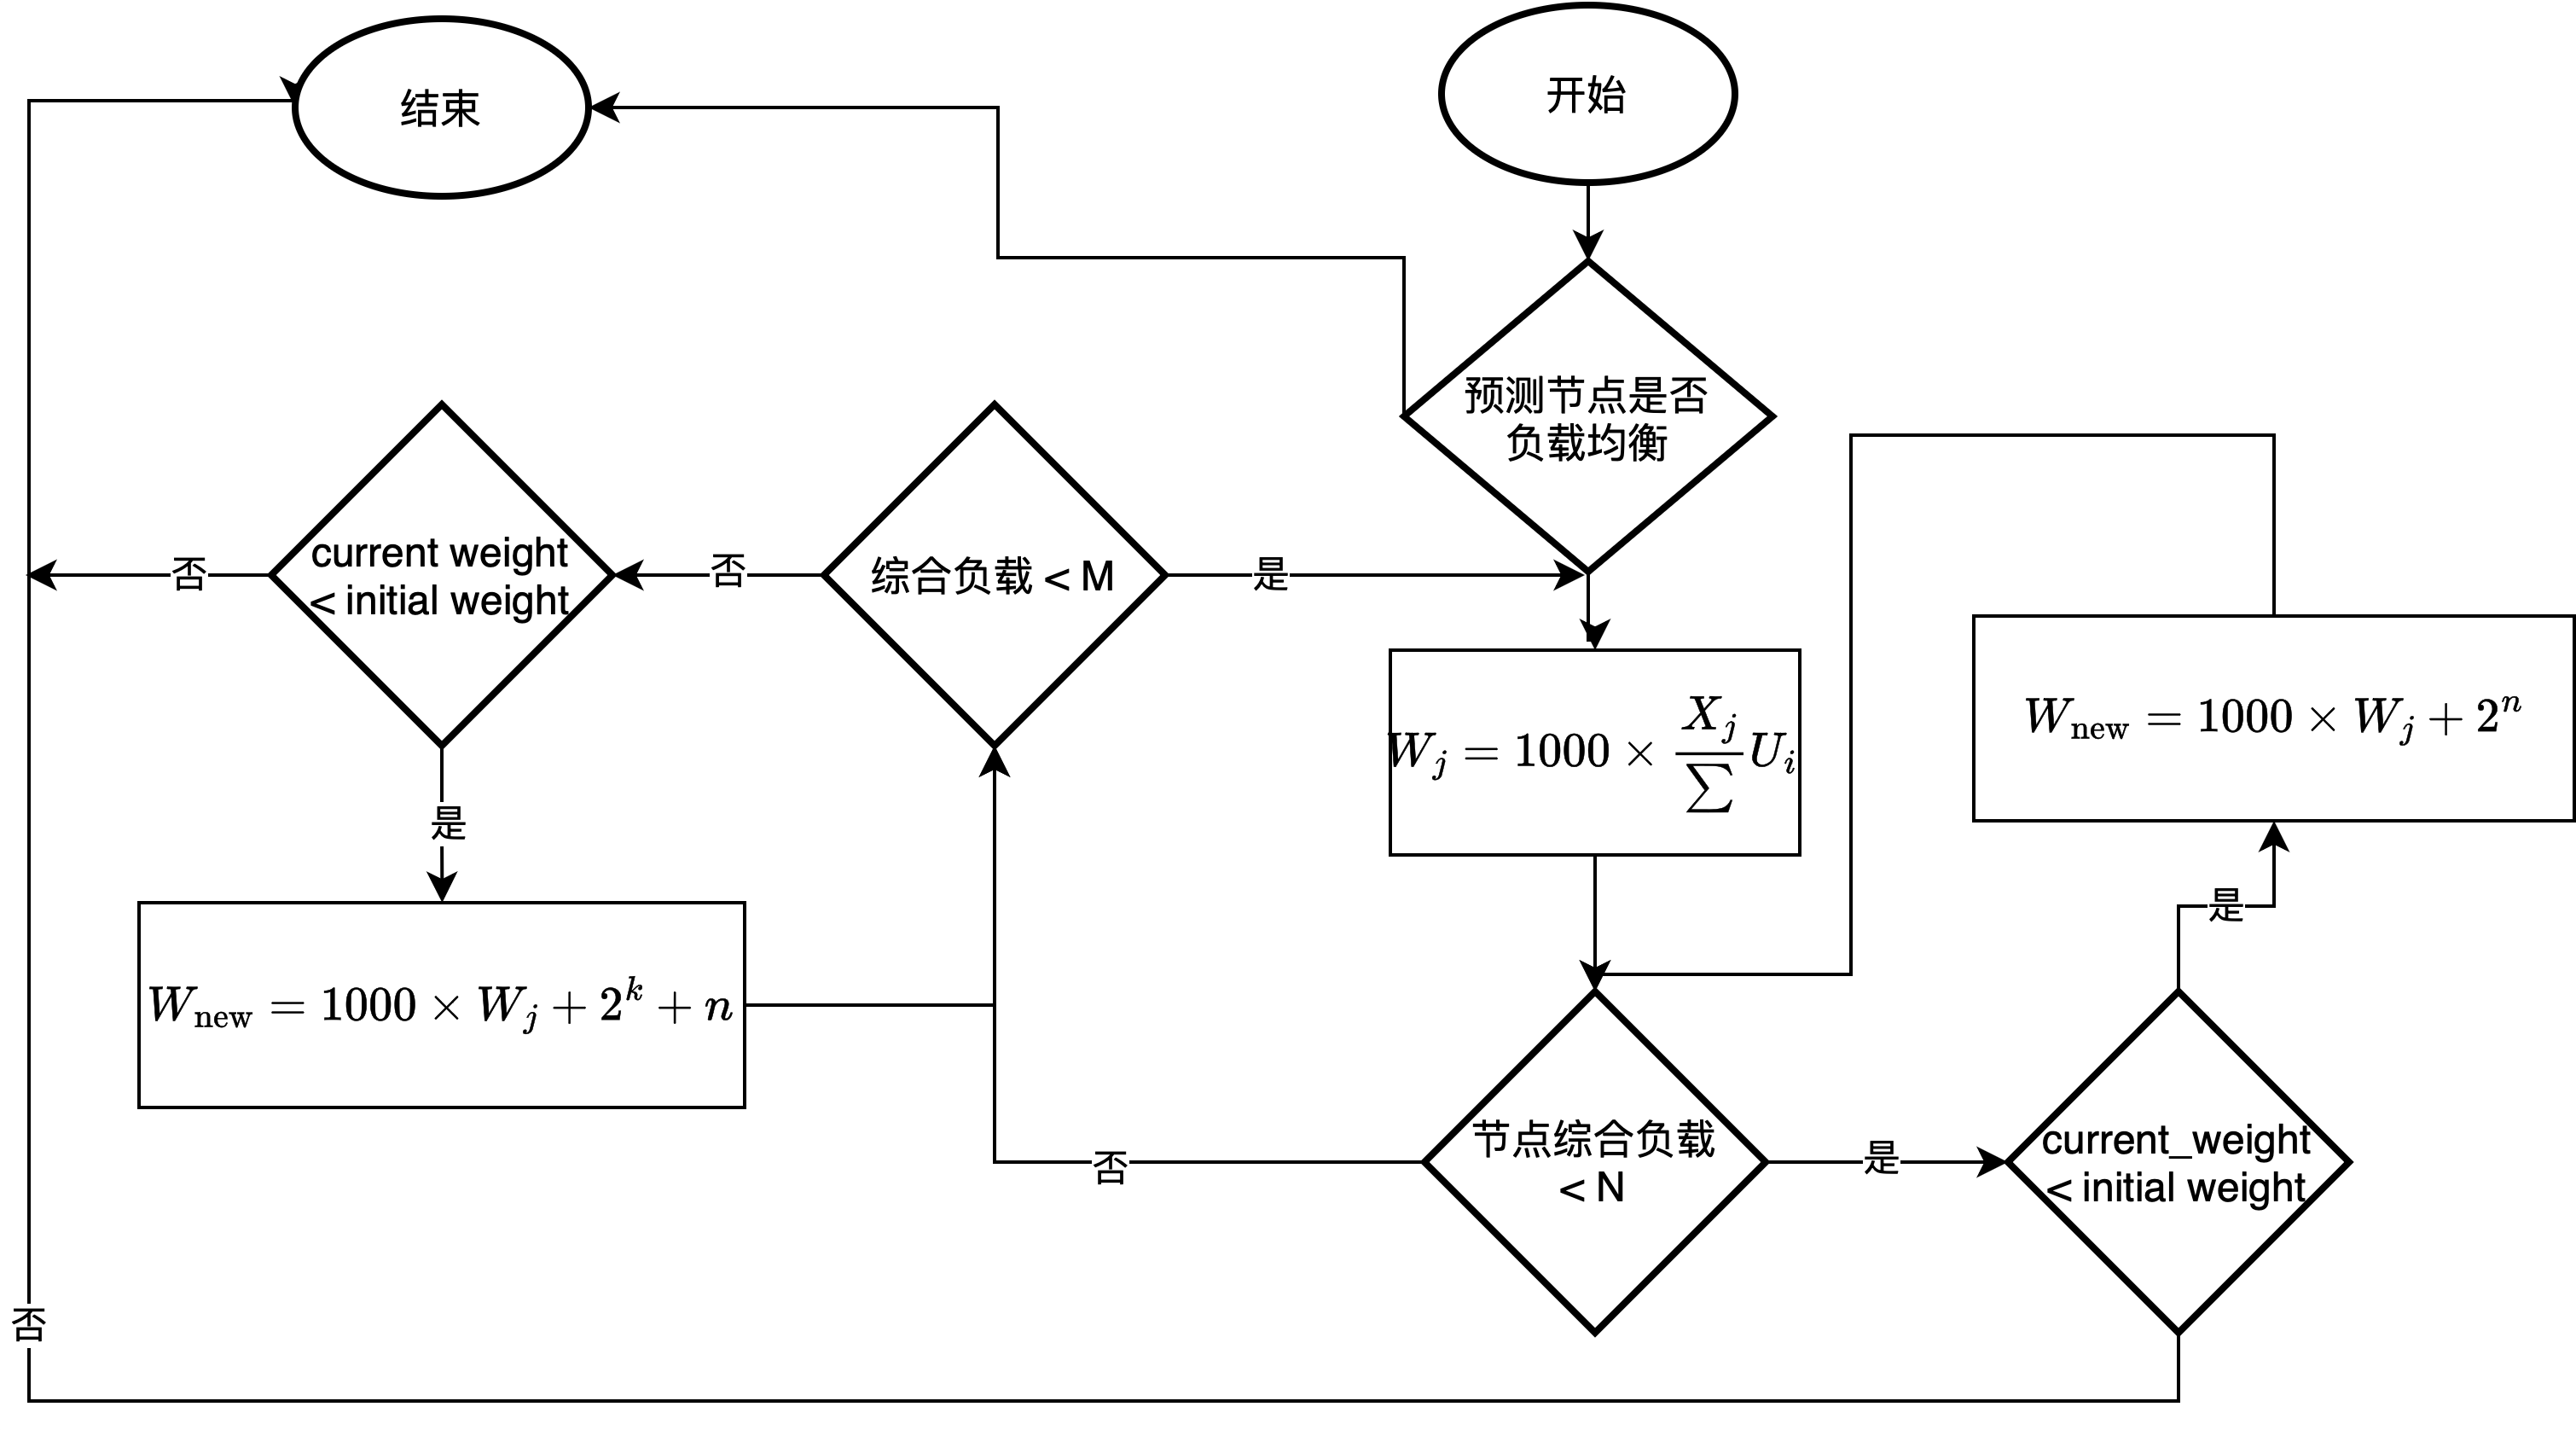
\includegraphics[width=\textwidth]{figures/change_weight.png}
	\caption{基于拥塞控制思想的权重调整流程}
	\label{contral_weight}
\end{figure}

\section{本章总结}

在本章中,通过研究常规的动态负载均衡方案的不足,提出了与预测模型相结合的动态负载均衡方案。
其中包含两个阶段,初期阶段和预测阶段,很好的解决了改进算法在没有数据时的负载均衡方案,提出了收集周期 $T$ 和初期阶段的初始权重,和调整权重的阈值 $N$,
同时借鉴了 TCP Reno 方案优化了负载均衡器调整权重时的阻塞情况。
